\hypertarget{seccion:IniciarSesion}{\vspace{1pt}}
\section{Marco Teórico}

\subsection{Big Data}
El término Big Data se refiere a cantidades enormes de información, por ejemplo, la cantidad de información que se produce todos los días con el uso de una red social como Facebook, o la cantidad de datos que producen computadoras y dispositivos electrónicos que se auto monitorean mediante sensores. Esos volúmenes masivos de datos pueden ser utilizados para extraer conocimiento de ellos, y posteriormente atacar problemas que no sería posible resolver sin el Big Data.

\subsubsection{Las 3 Vs del Big Data}
Al ser el Big Data un concepto emergente y relativamente nuevo, se han tenido ciertas dificultades para definirlo de manera uniforme. Debido a las dimensiones de todo lo que conlleva entender Big Data, resultó conveniente entre los estudiosos del tema definir y acentuar las magnitudes que lo definen. Estas magnitudes se conocen como las 3 Vs del Big Data.

\begin{enumerate}
	\item \textbf{Volumen:} Con Big Data, se tendrán que procesar enormes volúmenes de información. Este punto es importante ya que el crecimiento de la nececidad de almacenamiento de datos en el mundo moderno, crece de forma exponencial.
	\item \textbf{Velocidad:} Usando Big Data, se abre la posibilidad de acceso y flujo de datos a velocidades que no se podrían conseguir de manera convencional.
	\item \textbf{Variedad:} Procesamiento de datos de naturaleza heterogénea, es decir, múltiples tipos de datos.
\end{enumerate}

\subsubsection{Casos de uso del Big Data}

\begin{UClist}
	\UCli \textbf{Desarrollo de productos:} Compañías como Netflix y Procter \& Gamble utilizan el Big Data para anticiparse a la demanda de los consumidores de sus productos. Utilizan modelos predictivos para sus nuevos productos clasificando atributos clave de sus anteriores productos modelando las relaciones entre esos atributos.
	\UCli \textbf{Mantenimiento predictivo:} Se pueden predecir fallas mecánicas en maquinaria que de otra forma quedarían fácilmente ignoradas. Mejorando así ampliamente la calidad y el costo del mantenimiento de dichos equipos.
	\UCli \textbf{Experiencia de usuario:} El uso de Big Data permite recopilar toda la información sobre el usuario y utilizarla a favor de su experiencia en un sitio o aplicación. Por ejemplo, sus búsquedas frecuentes, los sitios que visita, etc. Para de esta manera empezar a hacerle ofertas o anuncios personalizados, según sus intereses particulares.
	\UCli \textbf{Machine Learning:} Actualmente el machine learning es un área de mucho auge, ya que permite entrenar a las computadoras mediante conjuntos de datos de entrenamiento en lugar de programarlas. El Big Data facilita esa tarea.
\end{UClist}

\subsection{Minería de datos}
La minería de datos es el proceso de generar conocimiento a partir de un conjunto de información de gran tamaño. Para generar ese conocimiento se utilizan diferentes técnicas de análisis que detectan patrones y tendencias en la información que se está procesando. Si se intentara utilizar algún método de análisis tradicional, sería muy complicado o incluso imposible a veces encontrar patrones y tendencias útiles, ya que es muy probable que dentro de los datos existan relaciones muy complejas o simplemente la cantidad de datos sea demasiado grande.\\

La minería de datos puede utilizarse en escenarios como los que se enuncian a continuación: \\
\begin{UClist}
	\UCli \textbf{Pronóstico:} Predicción de datos y eventos que vendrán a futuro a partir del comportamiento de conjuntos de datos que se tienen en el presente. Por ejemplo, predicción de ventas y tendencias de compra.
	\UCli \textbf{Riesgo y probabilidad:} Es un escenario muy común dentro de los negocios de Bussiness Intelligence. Por ejemplo, se llega a utilizar para encontrar puntos de equilibrio probable para escenarios de riesgo.
	Elección de los mejores clientes para la distribución de correo directo, determinación del punto de equilibrio probable para los escenarios de riesgo, y asignación de probabilidades a diagnósticos y otros resultados.
	\UCli \textbf{Recomendaciones:} Muy utilizado en sistemas como MercadoLibre o Amazon, en módulos que toman la información de búsqueda de cada usuario, la procesan y le arrojan recomendaciones de productos o servicios.
	\UCli \textbf{Búsqueda de secuencias:} Al igual que el escenario de \textbf{recomendaciones}, se utiliza mucho en sistemas de venta de artículos por internet. Se analiza el orden de los artículos que se meten a un carrito de compra para poder hacer predicciones útiles y generar conocimiento.
	\UCli \textbf{Agrupación:} Clasificación de los elementos de un conjunto de información para el posterior análisis de sus afinidades.
\end{UClist}

\subsection{Árboles de decisión}
Un árbol de decisión es un modelo de predicción que apoya al proceso de toma de decisiones. Esta herramienta tiene un campo de aplicación extremadamente amplio, pudiendo ir desde el área de finanzas hasta el área del aprendizaje de máquina. A partir de un conjunto de datos de entrada, se construyen los caminos, dentro del árbol, que llevarán a cada una de las decisiones posibles.\\

Los árboles de decisión están formados por los siguientes elementos:\\

\begin{enumerate}
	\item \textbf{Nodos:} Un nodo es un punto del proceso en el que de acuerdo a ciertas condiciones o decisiones se redefine el rumbo del camino. Existen dos tipos de nodo:
	\begin{enumerate}
		\item \textbf{Nodo de decisión:} Es un nodo en el cual se toma una decisión consciente de acuerdo a las necesidades del problema en cuestión. Estos nodos se representan con un cuadrado.
		\item \textbf{Nodo de incertidumbre: } Es un nodo en el que actúan las probabilidades y la heurística para definir el rumbo que tomará el camino que se hará dentro del árbol. Estos nodos se representan con un círculo
	\end{enumerate}
	\item \textbf{Ramas:} Una rama es una de las respuestas o acciones que se toman a partir de la pregunta o escenario que se presentó en un nodo del cual salió esa rama. Una rama es el camino a otro nodo o escenario resultado de la decisión o evento que definió la rama. Este elemento se representa con una línea.
	\item \textbf{Hojas:} Son escenarios finales, ya clasificados. No tienen ramificaciones, y son el resultado final de seguir un camino de decisiones, acciones y probabilidades. Este elemento se representa con un triángulo.
\end{enumerate}

\begin{figure}[!htbp]
	\hypertarget{fig:arbol-decision-ejemplo}{\hspace{1pt}}
	\begin{center}
		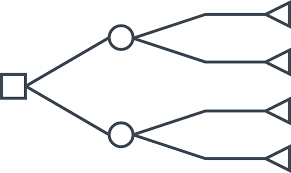
\includegraphics[height=0.3\textheight]{capitulo2/images/arbol-decision-ejemplo.png}
		\caption{Representación general de un árbol de decisión}
		\label{fig:arbol-decision-ejemplo}
	\end{center}
\end{figure}

\newpage
\subsection{ID3 (Iterative Dichotomiser 3)} \label{id3}

El algoritmo ID3 es uno de los algoritmos que utilizan árboles de decisión más populares. ID3 genera un árbol a partir de un conjunto de datos llamado \textbf{tabla de inducción}. Es útil para hacer toma de decisiones en escenarios binarios, es decir, que tienen 2 posibilidades finales.\\

El resultado de la ejecución de este algoritmo puede expresarse como un conjunto de reglas \textbf{\textit{si-entonces}}.

\subsubsection{Entropía}
La entropía es la medida de la aleatoriedad. En otras palabras, la medidad e la impredictibilidad. La entropía es más alta cuando todos los eventos posibles en un escenario son igualmente probables, por ejemplo, al tirar una moneda al aire, se tiene 50\% de probabilidad de que caiga cara y 50\% de probabilidad de que caiga cruz, por lo que la entropía es de 1. Este parámetro comienca a decrecer cuando hay una probabilidad o probabilidades que parezcan aplastantes sobre las otras. Las fórmulas para calcular la entropía y la ganancia son las siguiente:\\

\begin{figure}[!htbp]
	\hypertarget{fig:formula-entropia}{\hspace{1pt}}
	\begin{center}
		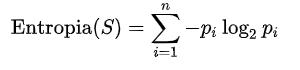
\includegraphics{capitulo2/images/formula-entropia.png}
		\caption{Fórmula para calcular la entropía.}
		\label{fig:formula-entropia}
	\end{center}
\end{figure}

\begin{figure}[!htbp]
	\hypertarget{fig:formula-ganancia}{\hspace{1pt}}
	\begin{center}
		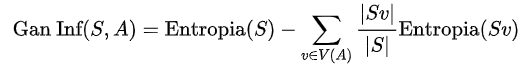
\includegraphics{capitulo2/images/formula-ganancia.png}
		\caption{Fórmula para calcular la ganancia.}
		\label{fig:formula-ganancia}
	\end{center}
\end{figure}

\subsubsection{Ejecución del algoritmo ID3} \label{ejecucionID3}

Para ilustrar el funcionamiento del algoritmo ID3, utilizaremos la siguiente tabla de inducción que contiene información sobre factores que influyen al tomar la decisión de si un partido de tenis debería o no debería jugarse:

\begin{table}[!hb]
	\begin{center}
		\label{tab:tablaInduccionID3}
		\begin{tabular}{c|c|c|c|c|c}
			\textbf{Día} & \textbf{Aspecto} & \textbf{Temperatura} & \textbf{Humedad} & \textbf{Viento} & \textbf{Decisión}\\
			\hline
			1 & Soleado & Caluroso & Alta & Ligero & No\\
			2 & Soleado & Caluroso & Alta & Fuerte & No\\
			3 & Nublado & Caluroso & Alta & Ligero & Sí\\
			4 & Lluvioso & Templado & Alta & Ligero & Sí\\
			5 & Lluvioso & Fresco & Normal & Ligero & Sí\\
			6 & Lluvioso & Fresco & Normal & Fuerte & No\\
			7 & Nublado & Fresco & Normal & Fuerte & Sí\\
			8 & Soleado & Templado & Alta & Ligero & No\\
			9 & Soleado & Fresco & Normal & Ligero & Sí\\
			10 & Lluvioso & Templado & Normal & Ligero & Sí\\
			11 & Soleado & Templado & Normal & Fuerte & Sí\\
			12 & Nublado & Templado & Alta & Fuerte & Sí\\
			13 & Nublado & Caluroso & Normal & Ligero & Sí\\
			14 & Lluvioso & Templado & Alta & Fuerte & No\\
		\end{tabular}
	\end{center}
	\caption{Tabla de inducción para juegos de tenis ID3.}
\end{table}

Necesitaremos de la \refIU{fig:formula-entropia}{fórmula para calcular la entropía} y de la \refIU{fig:formula-ganancia}{fórmula para calcular la ganancia} para poder proceder con la ejecución del algoritmo.\\

\begin{UClist}
	\UCli Primeramente se calcula la entropía. La columna de \textbf{Decisión} consta de 14 instancias e incluye dos posibles valores: \textbf{sí} y \textbf{no}. Hay 9 decisiones con la etiqueta \textbf{sí} y 5 con la etiqueta \textbf{no}. Utilizando la fórmula de la entropía, se encuentra que el resultado es de \emph{0.940}.\\
	\UCli Después de los 5 factores disponibles, se busca el factor más dominante para tomar la decisión. Utilizando la fórmula de la ganancia tomando como parámetros la entropía de la columna \textbf{Decisión} y \textbf{Viento}.\\
	\UCli El atributo de viento tiene dos posibles valores: \textbf{fuerte} y \textbf{ligero}. Y al reflejar estos dos posibles valores en la fórmula, ésta se vería más o menos así: \emph{Ganancia(Decisión, Viento) = Entropía(Decisión) - [p(Decisión, Viento = Ligero)*Entropía(Decisión, Viento = Ligero)]-[p(Decisión, Viento = Fuerte)*Entropía(Decisión, Viento = Fuerte)]}.\\
	\UCli Ahora se calcula \emph{(Decisión, Viento = Ligero)} y \emph{(Decisión, Viento = Fuerte)} respectivamente.\\

	\begin{table}[!hb]
		\begin{center}
			\label{tab:tablaInduccionVientoLigero}
			\begin{tabular}{c|c|c|c|c|c}
				\textbf{Día} & \textbf{Aspecto} & \textbf{Temperatura} & \textbf{Humedad} & \textbf{Viento} & \textbf{Decisión}\\
				\hline
				1 & Soleado & Caluroso & Alta & Ligero & No\\
				3 & Nublado & Caluroso & Alta & Ligero & Sí\\
				4 & Lluvioso & Templado & Alta & Ligero & Sí\\
				5 & Lluvioso & Fresco & Normal & Ligero & Sí\\
				8 & Soleado & Templado & Alta & Ligero & No\\
				9 & Soleado & Fresco & Normal & Ligero & Sí\\
				10 & Lluvioso & Templado & Normal & Ligero & Sí\\
				13 & Nublado & Caluroso & Normal & Ligero & Sí\\
			\end{tabular}
		\end{center}
		\caption{Tabla de para el factor de decisión \emph{Viento Ligero}.}
	\end{table}

	Dentro de la tabla de viento ligero hay 8 instancias en total, de las cuales 2 tienen la decisión final \textbf{no} y 6 tienen la decisión final \textbf{sí}. Al introducir estos datos en la \refIU{fig:formula-entropia}{fórmula de la entropía}, y obtenemos una entropía de \emph{0.811}.\\

	\newpage
	\begin{table}[!hb]
		\begin{center}
			\label{tab:tablaInduccionVientoFuerte}
			\begin{tabular}{c|c|c|c|c|c}
				\textbf{Día} & \textbf{Aspecto} & \textbf{Temperatura} & \textbf{Humedad} & \textbf{Viento} & \textbf{Decisión}\\
				\hline
				2 & Soleado & Caluroso & Alta & Fuerte & No\\
				6 & Lluvioso & Fresco & Normal & Fuerte & No\\
				7 & Nublado & Fresco & Normal & Fuerte & Sí\\
				11 & Soleado & Templado & Normal & Fuerte & Sí\\
				12 & Nublado & Templado & Alta & Fuerte & Sí\\
				14 & Lluvioso & Templado & Alta & Fuerte & No\\
			\end{tabular}
		\end{center}
		\caption{Tabla de para el factor de decisión \emph{Viento Fuerte}.}
	\end{table}

	En la tabla de viento fuerte encontramos 6 instancias divididas en 2 partes iguales: 3 tienen la decisión final \textbf{sí} y 3 tienen la decisión final \textbf{no}. Al sustituir estos datos en la \refIU{fig:formula-entropia}{fórmula de la entropía}, obtenemos una entropía de \emph{1}.\\

	\UCli Ahora que tenemos esos dos valores, podemos volver a la ecuación de la ganancia. El resultado queda expresado como \emph{Ganancia(Decisión, Viento) = 0.940-[(8/14)*0.811]-[(6/14)*1] = 0.048}.\\

	\UCli En este punto se ha concluido ya el cálculo para el factor de decisión \emph{Viento}. Ahora se necesita hacer lo mismo para todas las demas colúmnas/factores.\\

	\UCli A modo de resumen:

	\begin{enumerate}
		\item Ganancia(Decisión, Aspecto) = 0.246
		\item Ganancia(Decisión, Temperatura) = 0.029
		\item Ganancia(Decisión, Humedad) = 0.151
	\end{enumerate}

	\UCli Como podemos ver, el factor de decisión \emph{Aspecto} es el que produce el valor de ganancia más alto. Por tal motivo, ese factor de decisión será el nodo raíz del árbol de decisión.\\

	\UCli Ahora debemos probar todos los valores posibles que tiene el factor de decisión \emph{Aspecto}:\\

	\UCli Aspecto Nublado\\
	\begin{table}[H]
		\begin{center}
			\label{tab:tablaInduccionAspectoNublado}
			\begin{tabular}{c|c|c|c|c|c}
				\textbf{Día} & \textbf{Aspecto} & \textbf{Temperatura} & \textbf{Humedad} & \textbf{Viento} & \textbf{Decisión}\\
				\hline
				3 & Nublado & Caluroso & Alta & Ligero & Sí\\
				7 & Nublado & Fresco & Normal & Fuerte & Sí\\
				12 & Nublado & Templado & Alta & Fuerte & Sí\\
				13 & Nublado & Caluroso & Normal & Ligero & Sí\\
			\end{tabular}
		\end{center}
		\caption{Tabla de días con aspecto \emph{nublado}.}
	\end{table}

	Podemos observar que siempre que el aspecto del día sea \textbf{nublado}, la decisión final sería \textbf{sí}.\\

	\UCli Aspecto Soleado\\
	\begin{table}[H]
		\begin{center}
			\label{tab:tablaInduccionAspectoSoleado}
			\begin{tabular}{c|c|c|c|c|c}
				\textbf{Día} & \textbf{Aspecto} & \textbf{Temperatura} & \textbf{Humedad} & \textbf{Viento} & \textbf{Decisión}\\
				\hline
				1 & Soleado & Caluroso & Alta & Ligero & No\\
				2 & Soleado & Caluroso & Alta & Fuerte & No\\
				8 & Soleado & Templado & Alta & Ligero & No\\
				9 & Soleado & Fresco & Normal & Ligero & Sí\\
				11 & Soleado & Templado & Normal & Fuerte & Sí\\
			\end{tabular}
		\end{center}
		\caption{Tabla días con aspecto \emph{soleado}.}
	\end{table}

	En esta tabla tenemos 5 instancias para el aspecto \textbf{soleado}. Hay 3 de esas instancias que tienen como decisión final \textbf{sí} y 2 que tienen \textbf{no}. Por lo que los valores de ganancia del factor de decisión \textbf{Aspecto Soleado} con respecto a todos los demás factores de decisión quedarán de la siguiente manera:\\

	\begin{enumerate}
		\item Ganancia(Aspecto = Soleado, Temperatura) = 0.570
		\item Ganancia(Aspecto = Soleado, Humedad) = 0.970
		\item Ganancia(Aspecto = Soleado, Viento) = 0.019
	\end{enumerate}

	En este punto, la humedad es el factor de decisión con mayor ganancia cuando el aspecto del día es soleado. Por lo que debemos probar todos los valores posibles para el factor de decisión \emph{humedad}.\\

	\begin{table}[H]
		\begin{center}
			\label{tab:tablaInduccionAspectoSoleadoHumedadAlta}
			\begin{tabular}{c|c|c|c|c|c}
				\textbf{Día} & \textbf{Aspecto} & \textbf{Temperatura} & \textbf{Humedad} & \textbf{Viento} & \textbf{Decisión}\\
				\hline
				1 & Soleado & Caluroso & Alta & Ligero & No\\
				2 & Soleado & Caluroso & Alta & Fuerte & No\\
				8 & Soleado & Templado & Alta & Ligero & No\\
			\end{tabular}
		\end{center}
		\caption{Tabla días con aspecto \emph{soleado} y humedad \emph{alta}.}
	\end{table}

	La decisión siempre será \textbf{no} cuando la humedad sea \textbf{alta}.\\

	\begin{table}[H]
		\begin{center}
			\label{tab:tablaInduccionAspectoSoleadoHumedadNormal}
			\begin{tabular}{c|c|c|c|c|c}
				\textbf{Día} & \textbf{Aspecto} & \textbf{Temperatura} & \textbf{Humedad} & \textbf{Viento} & \textbf{Decisión}\\
				\hline
				9 & Soleado & Fresco & Normal & Ligero & Sí\\
				11 & Soleado & Templado & Normal & Fuerte & Sí\\
			\end{tabular}
		\end{center}
		\caption{Tabla días con aspecto \emph{soleado} y humedad \emph{normal}.}
	\end{table}

	Por otro lado, la decisión siempre será \textbf{sí} cuando la humedad es \textbf{normal}.\\

	De lo anterior concluimos que deberemos verificar la humedad y decidir si el aspecto del día es \textbf{soleado}.\\

	\UCli Aspecto Lluvioso\\
	\begin{table}[H]
		\begin{center}
			\label{tab:tablaInduccionAspectoLluvioso}
			\begin{tabular}{c|c|c|c|c|c}
				\textbf{Día} & \textbf{Aspecto} & \textbf{Temperatura} & \textbf{Humedad} & \textbf{Viento} & \textbf{Decisión}\\
				\hline
				4 & Lluvioso & Templado & Alta & Ligero & Sí\\
				5 & Lluvioso & Fresco & Normal & Ligero & Sí\\
				6 & Lluvioso & Fresco & Normal & Fuerte & No\\
				10 & Lluvioso & Templado & Normal & Ligero & Sí\\
				14 & Lluvioso & Templado & Alta & Fuerte & No\\
			\end{tabular}
		\end{center}
		\caption{Tabla de días con aspecto \emph{lluvioso}.}
	\end{table}

	Al evaluar los valores de ganancia de los días con aspecto \textbf{lluvioso} con respecto a los demás factores de decisión, se encuentra que el factor que genera una mayor ganancia es el viento. Por lo cual se tienen que checar todos los posibles valores de ese factor de decisión.\\

	\begin{table}[H]
		\begin{center}
			\label{tab:tablaInduccionAspectoLluviosoVientoLigero}
			\begin{tabular}{c|c|c|c|c|c}
				\textbf{Día} & \textbf{Aspecto} & \textbf{Temperatura} & \textbf{Humedad} & \textbf{Viento} & \textbf{Decisión}\\
				\hline
				4 & Lluvioso & Templado & Alta & Ligero & Sí\\
				5 & Lluvioso & Fresco & Normal & Ligero & Sí\\
				10 & Lluvioso & Templado & Normal & Ligero & Sí\\
			\end{tabular}
		\end{center}
		\caption{Tabla de días con aspecto \emph{lluvioso} y con viento \emph{ligero}.}
	\end{table}

	De la tabla de aspecto \textbf{lluvioso} y viento \textbf{ligero} podemos deducir que siempre que existan estas dos condiciones al mismo tiempo, la decisión final será \textbf{sí}.\\

	\begin{table}[H]
		\begin{center}
			\label{tab:tablaInduccionAspectoLluvioso}
			\begin{tabular}{c|c|c|c|c|c}
				\textbf{Día} & \textbf{Aspecto} & \textbf{Temperatura} & \textbf{Humedad} & \textbf{Viento} & \textbf{Decisión}\\
				\hline
				6 & Lluvioso & Fresco & Normal & Fuerte & No\\
				14 & Lluvioso & Templado & Alta & Fuerte & No\\
			\end{tabular}
		\end{center}
		\caption{Tabla de días con aspecto \emph{lluvioso}.}
	\end{table}

	De la tabla de aspecto \textbf{lluvioso} y viento \textbf{fuerte} podemos deducir que siempre que existan estas dos condiciones al mismo tiempo, la decisión final será \textbf{no}.\\

	\UCli Finalmente la construcción de este árbol de decisión es la siguiente:

	\begin{figure}[H]
		\hypertarget{fig:arbol-decision-final}{\hspace{1pt}}
		\begin{center}
			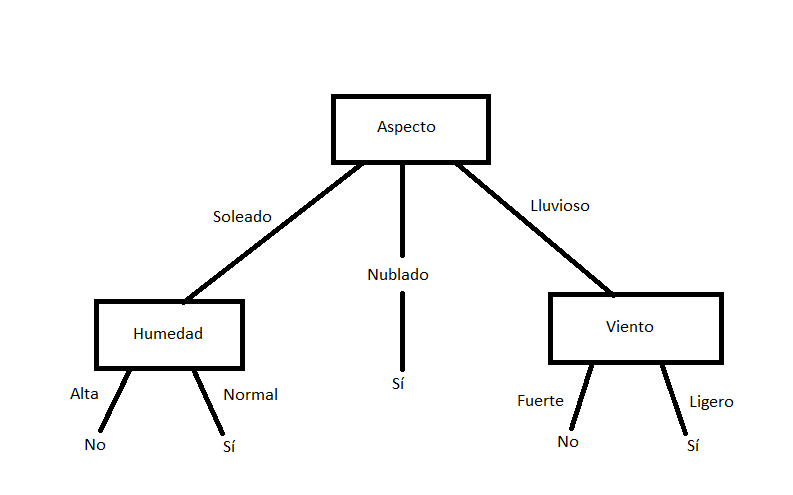
\includegraphics{capitulo2/images/arbol-decision-final.png}
			\caption{Árbol de decisión resultante.}
			\label{fig:arbol-decision-final}
		\end{center}
	\end{figure}

\end{UClist}


\subsection{C4.5} \label{c4.5}
El algoritmo C4.5 es la evolución del algoritmo ID3. Éste genera un árbol de decisión a partir de un conjunto de dstos de entrada de manera recursiva, al igual que su precursor. Sin embargo, aunque ID3 y C4.5 son algoritmos muy semejantes, existen ciertas diferencias:\\

\begin{UClist}
	\UCli C4.5 permite trabajar con valores continuos, mientras que ID3 solamente trabaja con valores discretos.\\
	\UCli Los árboles de C4.5 son más compactos, y esto se debe a que cada nodo hoja engloba un conjunto de clases y no una sola clase particular.\\
	\UCli C4.5 es más eficiente computacionalmente hablando.\\
	\UCli C4.5 utiliza un nuevo parámetro llamado \textbf{Gain Ratio}, en lugar de la ganancia simple. Y este a su vez requiere de la ganancia y de otro parámetro nuevo llamado \textbf{SplitInfo} cuyas fórmulas se enuncian a continuación:
	
	\begin{figure}[H]
		\hypertarget{fig:formula-gainratio}{\hspace{1pt}}
		\begin{center}
			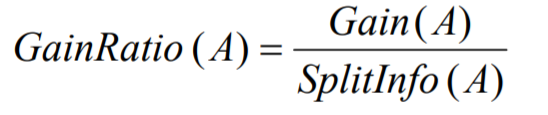
\includegraphics[width=0.5\textwidth]{capitulo2/images/formula-gainratio.png}
			\caption{Fórmula para obtener el Gain Ratio}
			\label{fig:formula-gainratio}
		\end{center}
	\end{figure}

	\begin{figure}[H]
		\hypertarget{fig:formula-splitinfo}{\hspace{1pt}}
		\begin{center}
			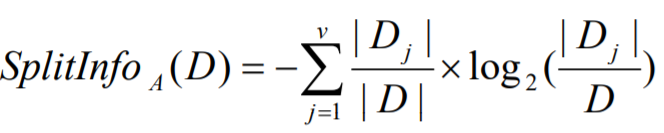
\includegraphics[width=0.5\textwidth]{capitulo2/images/formula-splitinfo.png}
			\caption{Fórmula para obtener SplitInfo}
			\label{fig:formula-splitinfo}
		\end{center}
	\end{figure}

\end{UClist}

\subsubsection{Ejecución del algoritmo C4.5}
Para mostrar la forma en la que se ejecuta el algoritmo C4.5 y los pasos que se deben llevar a cabo, se utilizará la siguiente tabla de inducción:

\begin{table}[H]
	\begin{center}
		\label{tab:tablaInduccionC4.5}
		\begin{tabular}{c|c|c|c|c|c}
			\textbf{Día} & \textbf{Aspecto} & \textbf{Temperatura} & \textbf{Humedad} & \textbf{Viento} & \textbf{Decisión}\\
			\hline
			1 & Soleado & 85 & 85 & Ligero & No\\
			2 & Soleado & 80 & 90 & Fuerte & No\\
			3 & Nublado & 83 & 78 & Ligero & Sí\\
			4 & Lluvioso & 70 & 96 & Ligero & Sí\\
			5 & Lluvioso & 68 & 80 & Ligero & Sí\\
			6 & Lluvioso & 65 & 70 & Fuerte & No\\
			7 & Nublado & 64 & 65 & Fuerte & Sí\\
			8 & Soleado & 72 & 95 & Ligero & No\\
			9 & Soleado & 69 & 70 & Ligero & Sí\\
			10 & Lluvioso & 75 & 80 & Ligero & Sí\\
			11 & Soleado & 75 & 70 & Fuerte & Sí\\
			12 & Nublado & 72 & 90 & Fuerte & Sí\\
			13 & Nublado & 81 & 75 & Ligero & Sí\\
			14 & Lluvioso & 80 & 80 & Fuerte & No\\
		\end{tabular}
	\end{center}
	\caption{Tabla de inducción para juegos de tenis C4.5.}
\end{table}

\begin{UClist}
	\UCli Al igual que con el ejemplo \nameref{ejecucionID3}, lo primero que se hace es calcular la entropía general. Hay 15 instancias de las cuales 9 tienen una decisión final de \textbf{sí} y 5 tienen \textbf{no}. Al sustituir los valores correspondientes en la \refIU{fig:formula-entropia}{fórmula para calcular la entropía} el resultado que obtenemos es \emph{0.940}.\\

	\UCli En C4.5 se utilizan \textbf{Gain Ratios} (radios de ganancia), mientras que en ID3 se utilizan ganancias.\\

	\UCli Empezaremos por analizar el atributo de \textbf{Viento}.\\

	Se tienen 8 instancias de \emph{viento ligero}, dos de ellas concluyen en un \textbf{no}, y las otras 6 concluyen en \textbf{sí} por lo que:\\

	\begin{enumerate}
		\item Entropía(Decisión, Viento = Ligero) = 0.811\\
		\item Entropía(Decisión, Viento = Fuerte) = 1\\
		\item Ganancia(Decisión, Viento) = 0.049\\
	\end{enumerate}

	Existen 6 instancias de viento fuerte por lo que:

	\begin{enumerate}
		\item SplitInfo(Decisión, Viento) = 0.985\\
		\item GainRatio(Decisión, Viento) = Gain(Decisión, Viento) / SplitInfo(Decision, Viento) = 0.049\\
	\end{enumerate}

	\UCli Continuamos analizando ahora el atributo \textbf{Aspecto}.\\

	Se tienen 5 instancias para el aspecto \emph{soleado}, de las cuales 3 concluyen en \textbf{no} y las otras 2 concluyen en \textbf{sí}. Calculando sus valores de entropías, ganancia, SplitInfo y GainRatio:\\

	\begin{enumerate}
		\item Entropía(Decisión, Aspecto = Soleado) = 0.970\\
		\item Entropía(Decisión, Aspecto = Nublado) = 0\\
		\item Entropía(Decisión, Aspecto = Lluvioso) = 0.970\\
		\item Ganancia(Decisión, Aspecto) = 0.246\\
		Hay 5 instancias para \emph{soleado}, 4 instancias para \emph{nublado} y 5 para \emph{lluvioso}, por lo que:\\
		\item SplitInfo(Decisión, Aspecto) = 1.577\\
		\item GainRatio(Decisión, Aspecto) = 0.155\\
	\end{enumerate}

	\UCli Procedemos a analizar el atributo de humedad. Cuyo caso es diferente al de los demás atributos, ya que este es un atributo continuo. Necesitamos convertir valoress continuos a valores nominales (como todos los demás atributos). C4.5 propone hacer una división binaria a partir de algún valor que podamos tomar como umbral. El umbral debe ser el valor que mayor ganancia ofrezca para ese atributo. Para esto, primero se deben ordenar las instancias de humedad de menor a mayor.\\

	\begin{table}[H]
		\begin{center}
			\label{tab:tablaInduccionC4.5Humedad}
			\begin{tabular}{c|c|c}
				\textbf{Día} & \textbf{Humedad} & \textbf{Decisión}\\
				\hline
				7 & 65 & Sí\\
				6 & 70 & No\\
				9 & 70 & Sí\\
				11 & 70 & Sí\\
				13 & 75 & Sí\\
				3 & 78 & Sí\\
				5 & 80 & Sí\\
				10 & 80 & Sí\\
				14 & 80 & No\\
				1 & 85 & No\\
				2 & 90 & No\\
				12 & 90 & Sí\\
				8 & 95 & No\\
				4 & 96 & Sí\\
			\end{tabular}
		\end{center}
		\caption{Tabla de l atributo \emph{humedad} ordenada de menor a mayor.}
	\end{table}

	Ahora debemos recorrer todos los valores de humedad y separar el conjunto de datos en dos partes. Se calcularán la \textbf{Ganancia} y el \textbf{GainRatio} y el valor que maximice la ganancia será el umbral.\\

	\begin{enumerate}
		\item Se propone 65 como umbral.
		\begin{enumerate}
			\item Entropía(Decisión, Humedad <= 65) = 0
			\item Entropía(Decisión, Humedad > 65) = 0.961
			\item Ganancia(Decisión, Humedad <> 65) = 0.048
			\item SplitInfo(Decisión, Humedad <> 65) = 0.371
			\item GainRatio(Decisión, Humedad <> 65) = 0.126\\
		\end{enumerate}
		\item Se propone 70 como umbral.
		\begin{enumerate}
			\item Entropía(Decisión, Humedad <= 70) = 0.811
			\item Entropía(Decisión, Humedad > 70) = 0.970
			\item Ganancia(Decisión, Humedad <> 70) = 0.014
			\item SplitInfo(Decisión, Humedad <> 70) = 0.863
			\item GainRatio(Decisión, Humedad <> 70) = 0.016\\
		\end{enumerate}
		\item Se propone 75 como umbral.
		\begin{enumerate}
			\item Entropía(Decisión, Humedad <= 75) = 0.721
			\item Entropía(Decisión, Humedad > 75) = 0.991
			\item Ganancia(Decisión, Humedad <> 75) = 0.045
			\item SplitInfo(Decisión, Humedad <> 75) = 0.940
			\item GainRatio(Decisión, Humedad <> 75) = 0.047\\
		\end{enumerate}
		\item Se continúa haciendo lo mismo para cada valor nuevo de humedad que se vaya encontrando en la tabla. Resumiendo:
		\item Ganancia(Decisión, Humedad <> 78) = 0.090
		\item Ganancia(Decisión, Humedad <> 80) = 0.107
		\item Ganancia(Decisión, Humedad <> 85) = 0.027
		\item Ganancia(Decisión, Humedad <> 90) = 0.016
	\end{enumerate}

	\UCli Como podemos ver, el valor que maximiza la ganancia es el de 80. Lo que significa que ahora se debe comparar los otros valores nominales con el valor 80 del atributo \emph{humedad} para crear una rama en nuestro árbol. De esta forma podemos resumir los resultados en la siguiente tabla:\\

	\begin{table}[H]
		\label{tab:tablaComparacionHumedadAtributos}
		\begin{center}
			\begin{tabular}{c|c|c}
				\textbf{Atributo} & \textbf{Ganancia} & \textbf{GainRatio}\\
				\hline
				Viento & 0.049 & 0.049\\
				Aspecto & 0.246 & 0.155\\
				Humedad <> 80 & 0.101 & 0.107\\
			\end{tabular}
			\caption{Comparación de las ganancias entre atributos.}
		\end{center}
	\end{table} 

	\UCli Al igual que en el ejemplo del algoritmo ID3, el atributo \textbf{aspecto} es el nodo raíz del árbol de decisión, por lo que ahora se deben analizar todos los posibles valores que puede adquirir dicho atributo.\\

	\UCli Aspecto Soleado.\\

	\begin{table}[H]
		\begin{center}
			\label{tab:tablaSoleadoC4.5}
			\begin{tabular}{c|c|c|c|c|c}
				\textbf{Día} & \textbf{Aspecto} & \textbf{Temperatura} & \textbf{Humedad} & \textbf{Viento} & \textbf{Decisión}\\
				\hline
				1 & Soleado & 85 & 85 & Ligero & No\\
				2 & Soleado & 80 & 90 & Fuerte & No\\
				8 & Soleado & 72 & 95 & Ligero & No\\
				9 & Soleado & 69 & 70 & Ligero & Sí\\
				11 & Soleado & 75 & 70 & Fuerte & Sí\\
			\end{tabular}
		\end{center}
		\caption{Tabla de inducción para el atributo \emph{Aspecto} con el valor \emph{Soleado}.}
	\end{table}

	Ya hemos dividido la humedad a partir de su punto de umbral que es 80. Podemos observar en la siguiente tabla que la decisión final será \textbf{no}, si la humedad es mayor a 80 y el aspecto del día es soleado. La decisión final será \textbf{sí}, si la humedad es menor o igual a 80 para un día soleado.\\

	\begin{table}[H]
		\begin{center}
			\label{tab:tablaNubladoC4.5}
			\begin{tabular}{c|c|c|c|c|c}
				\textbf{Día} & \textbf{Aspecto} & \textbf{Temperatura} & \textbf{Humedad} & \textbf{Viento} & \textbf{Decisión}\\
				\hline
				3 & Nublado & 83 & 78 & Ligero & Sí\\
				7 & Nublado & 64 & 65 & Fuerte & Sí\\
				12 & Nublado & 72 & 90 & Fuerte & Sí\\
				13 & Nublado & 81 & 75 & Ligero & Sí\\
			\end{tabular}
		\end{center}
		\caption{Tabla de inducción para el atributo \emph{Aspecto} con el valor \emph{Nublado}.}
	\end{table}

	Cuando el aspecto del día es \textbf{nublado}, no importa ninguna otra condición; ni temperatura, ni humedad. La decisión final siempre será \textbf{sí}.\\

	\begin{table}[H]
		\begin{center}
			\label{tab:tablaLluviosoC4.5}
			\begin{tabular}{c|c|c|c|c|c}
				\textbf{Día} & \textbf{Aspecto} & \textbf{Temperatura} & \textbf{Humedad} & \textbf{Viento} & \textbf{Decisión}\\
				\hline
				4 & Lluvioso & 70 & 96 & Ligero & Sí\\
				5 & Lluvioso & 68 & 80 & Ligero & Sí\\
				6 & Lluvioso & 65 & 70 & Fuerte & No\\
				10 & Lluvioso & 75 & 80 & Ligero & Sí\\
				14 & Lluvioso & 80 & 80 & Fuerte & No\\
			\end{tabular}
		\end{center}
		\caption{Tabla de inducción para el atributo \emph{Aspecto} con el valor \emph{Lluvioso}.}
	\end{table}

	Cuando el aspecto es \textbf{lluvioso}, la decisión será \textbf{sí} cuando el viento es ligero, y será \textbf{no} cuando sea fuerte.\\

	\UCli De todo lo anterior se concluye un árbol de decisión con la siguiente estructura:\\

	\begin{figure}[H]
		\hypertarget{fig:arbol-final-c45}{\hspace{1pt}}
		\begin{center}
			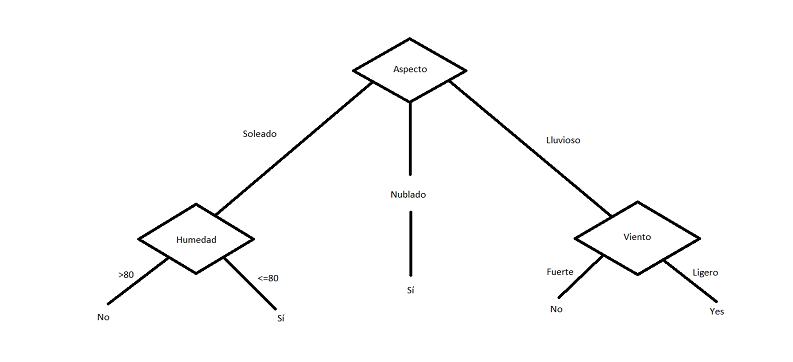
\includegraphics{capitulo2/images/arbol-final-c45.png}
			\caption{Arbol de decisión construido con C4.5.}
			\label{fig:arbol-final-c45}
		\end{center}
	\end{figure}

\end{UClist}

\subsection{Spark}
Es una herramienta de código abierto. Es un motor de análisis de datos unificado para Big Data y Machine Learning. 
\subsection{Hadoop}
Es un framework de software que soporta aplicaciones distribuidas bajo una licencia libre. Permite a las aplicaciones trabajar con miles de nodos y petabytes de datos. Hadoop se inspiró en los documentos Google para MapReduce y Google File System (GFS). Hadoop utiliza su propio sistema de archivos HDFS, que divide archivos grandes y los distribuye en diferentes nodos para su procesamiento.
% Para que la ELD pueda mantener actualizado el status de pago de los aspirantes que realizaron la operación en sucursal bancaria, es necesario que el \textbf{Contador General} actualice de forma manual dichos pagos, esto se logra con ayuda de
\begin{enumerate}
	\item Solicite administrar los pagos admisión seleccionando la opción \textbf{Administración de pagos} del menú \refIU{fig:menuPrincipalCG}{Menú del Contador General} y posteriormente la opción \textbf{Pagos Admisión} del menú \refIU{fig:menuPagosA}{Menú Pagos Admisión}.
	\item Se mostrará la pantalla \refIU{fig:ss}{Administrar Pagos Admisión}.
	\begin{figure}[!htbp]
		\hypertarget{fig:ss}{\hspace{1pt}}
		\begin{center}
			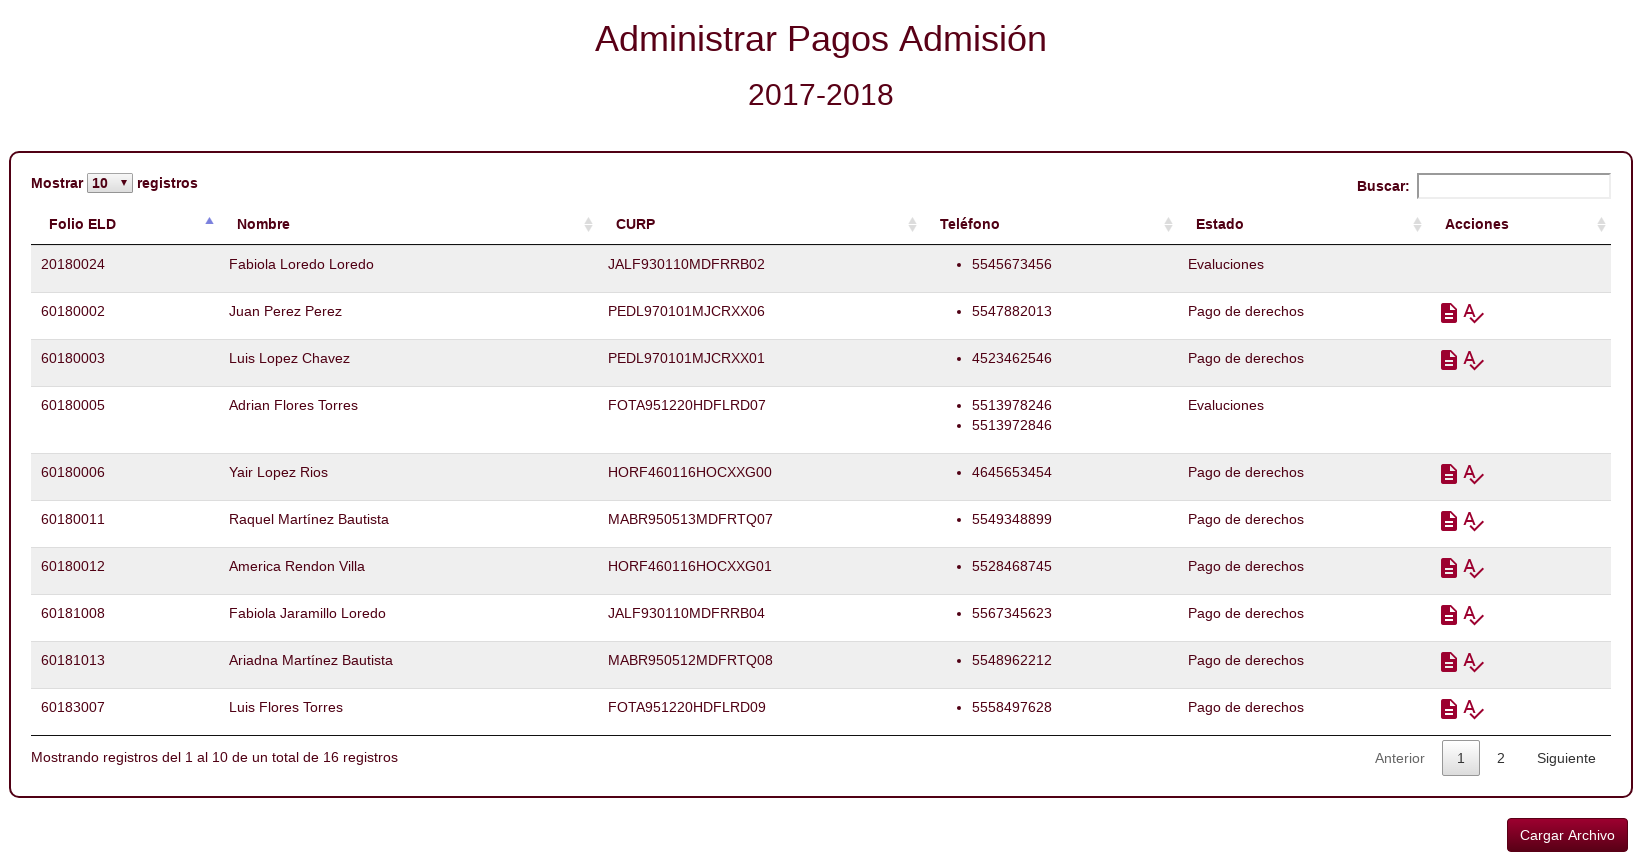
\includegraphics[height=0.3\textheight]{capitulo1/images/IU-APA.png}
			\caption{Administrar Pagos Admisión}
			\label{fig:ss}
		\end{center}
	\end{figure}

	
\end{enumerate}
	


\newpage
\begin{Errores}
	\error{El sistema muestra un mensaje indicando que falta información para realizar la operación.}
	{
		\begin{UClist}
			\UCli	Verifique que exista una convocatoria \textbf{Publicada}.
			\UCli	Verifique que exista un periodo de pagos.
			\UCli	Verifique que exista un periodo de pre-registro CENEVAL vigente.
		\end{UClist}
	}
	\error{El sistema muestra un mensaje indicando que no se ha realizado la asociación de fechas de CENEVAL y Psicométrico.}
	{
		\begin{UClist}
			\UCli	Verifique que la Coordinación de Control Escolar haya asociado las fechas CENEVAL y Psicométrico.
		\end{UClist}
	}
	

\end{Errores}
